% Options for packages loaded elsewhere
\PassOptionsToPackage{unicode}{hyperref}
\PassOptionsToPackage{hyphens}{url}
%
\documentclass[
  man,floatsintext]{apa6}
\usepackage{amsmath,amssymb}
\usepackage{lmodern}
\usepackage{iftex}
\ifPDFTeX
  \usepackage[T1]{fontenc}
  \usepackage[utf8]{inputenc}
  \usepackage{textcomp} % provide euro and other symbols
\else % if luatex or xetex
  \usepackage{unicode-math}
  \defaultfontfeatures{Scale=MatchLowercase}
  \defaultfontfeatures[\rmfamily]{Ligatures=TeX,Scale=1}
\fi
% Use upquote if available, for straight quotes in verbatim environments
\IfFileExists{upquote.sty}{\usepackage{upquote}}{}
\IfFileExists{microtype.sty}{% use microtype if available
  \usepackage[]{microtype}
  \UseMicrotypeSet[protrusion]{basicmath} % disable protrusion for tt fonts
}{}
\makeatletter
\@ifundefined{KOMAClassName}{% if non-KOMA class
  \IfFileExists{parskip.sty}{%
    \usepackage{parskip}
  }{% else
    \setlength{\parindent}{0pt}
    \setlength{\parskip}{6pt plus 2pt minus 1pt}}
}{% if KOMA class
  \KOMAoptions{parskip=half}}
\makeatother
\usepackage{xcolor}
\usepackage{graphicx}
\makeatletter
\def\maxwidth{\ifdim\Gin@nat@width>\linewidth\linewidth\else\Gin@nat@width\fi}
\def\maxheight{\ifdim\Gin@nat@height>\textheight\textheight\else\Gin@nat@height\fi}
\makeatother
% Scale images if necessary, so that they will not overflow the page
% margins by default, and it is still possible to overwrite the defaults
% using explicit options in \includegraphics[width, height, ...]{}
\setkeys{Gin}{width=\maxwidth,height=\maxheight,keepaspectratio}
% Set default figure placement to htbp
\makeatletter
\def\fps@figure{htbp}
\makeatother
\setlength{\emergencystretch}{3em} % prevent overfull lines
\providecommand{\tightlist}{%
  \setlength{\itemsep}{0pt}\setlength{\parskip}{0pt}}
\setcounter{secnumdepth}{-\maxdimen} % remove section numbering
% Make \paragraph and \subparagraph free-standing
\ifx\paragraph\undefined\else
  \let\oldparagraph\paragraph
  \renewcommand{\paragraph}[1]{\oldparagraph{#1}\mbox{}}
\fi
\ifx\subparagraph\undefined\else
  \let\oldsubparagraph\subparagraph
  \renewcommand{\subparagraph}[1]{\oldsubparagraph{#1}\mbox{}}
\fi
\newlength{\cslhangindent}
\setlength{\cslhangindent}{1.5em}
\newlength{\csllabelwidth}
\setlength{\csllabelwidth}{3em}
\newlength{\cslentryspacingunit} % times entry-spacing
\setlength{\cslentryspacingunit}{\parskip}
\newenvironment{CSLReferences}[2] % #1 hanging-ident, #2 entry spacing
 {% don't indent paragraphs
  \setlength{\parindent}{0pt}
  % turn on hanging indent if param 1 is 1
  \ifodd #1
  \let\oldpar\par
  \def\par{\hangindent=\cslhangindent\oldpar}
  \fi
  % set entry spacing
  \setlength{\parskip}{#2\cslentryspacingunit}
 }%
 {}
\usepackage{calc}
\newcommand{\CSLBlock}[1]{#1\hfill\break}
\newcommand{\CSLLeftMargin}[1]{\parbox[t]{\csllabelwidth}{#1}}
\newcommand{\CSLRightInline}[1]{\parbox[t]{\linewidth - \csllabelwidth}{#1}\break}
\newcommand{\CSLIndent}[1]{\hspace{\cslhangindent}#1}
\ifLuaTeX
\usepackage[bidi=basic]{babel}
\else
\usepackage[bidi=default]{babel}
\fi
\babelprovide[main,import]{english}
% get rid of language-specific shorthands (see #6817):
\let\LanguageShortHands\languageshorthands
\def\languageshorthands#1{}
% Manuscript styling
\usepackage{upgreek}
\captionsetup{font=singlespacing,justification=justified}

% Table formatting
\usepackage{longtable}
\usepackage{lscape}
% \usepackage[counterclockwise]{rotating}   % Landscape page setup for large tables
\usepackage{multirow}		% Table styling
\usepackage{tabularx}		% Control Column width
\usepackage[flushleft]{threeparttable}	% Allows for three part tables with a specified notes section
\usepackage{threeparttablex}            % Lets threeparttable work with longtable

% Create new environments so endfloat can handle them
% \newenvironment{ltable}
%   {\begin{landscape}\centering\begin{threeparttable}}
%   {\end{threeparttable}\end{landscape}}
\newenvironment{lltable}{\begin{landscape}\centering\begin{ThreePartTable}}{\end{ThreePartTable}\end{landscape}}

% Enables adjusting longtable caption width to table width
% Solution found at http://golatex.de/longtable-mit-caption-so-breit-wie-die-tabelle-t15767.html
\makeatletter
\newcommand\LastLTentrywidth{1em}
\newlength\longtablewidth
\setlength{\longtablewidth}{1in}
\newcommand{\getlongtablewidth}{\begingroup \ifcsname LT@\roman{LT@tables}\endcsname \global\longtablewidth=0pt \renewcommand{\LT@entry}[2]{\global\advance\longtablewidth by ##2\relax\gdef\LastLTentrywidth{##2}}\@nameuse{LT@\roman{LT@tables}} \fi \endgroup}

% \setlength{\parindent}{0.5in}
% \setlength{\parskip}{0pt plus 0pt minus 0pt}

% Overwrite redefinition of paragraph and subparagraph by the default LaTeX template
% See https://github.com/crsh/papaja/issues/292
\makeatletter
\renewcommand{\paragraph}{\@startsection{paragraph}{4}{\parindent}%
  {0\baselineskip \@plus 0.2ex \@minus 0.2ex}%
  {-1em}%
  {\normalfont\normalsize\bfseries\itshape\typesectitle}}

\renewcommand{\subparagraph}[1]{\@startsection{subparagraph}{5}{1em}%
  {0\baselineskip \@plus 0.2ex \@minus 0.2ex}%
  {-\z@\relax}%
  {\normalfont\normalsize\itshape\hspace{\parindent}{#1}\textit{\addperi}}{\relax}}
\makeatother

% \usepackage{etoolbox}
\makeatletter
\patchcmd{\HyOrg@maketitle}
  {\section{\normalfont\normalsize\abstractname}}
  {\section*{\normalfont\normalsize\abstractname}}
  {}{\typeout{Failed to patch abstract.}}
\patchcmd{\HyOrg@maketitle}
  {\section{\protect\normalfont{\@title}}}
  {\section*{\protect\normalfont{\@title}}}
  {}{\typeout{Failed to patch title.}}
\makeatother

\usepackage{xpatch}
\makeatletter
\xapptocmd\appendix
  {\xapptocmd\section
    {\addcontentsline{toc}{section}{\appendixname\ifoneappendix\else~\theappendix\fi\\: #1}}
    {}{\InnerPatchFailed}%
  }
{}{\PatchFailed}
\keywords{visual illusions, illusion game, pyllusion, illusion effect, personality\newline\indent Word count: 1156}
\usepackage{lineno}

\linenumbers
\usepackage{csquotes}
\usepackage[titles]{tocloft}
\cftpagenumbersoff{figure}
\renewcommand{\cftfigpresnum}{\itshape\figurename\enspace}
\renewcommand{\cftfigaftersnum}{.\space}
\setlength{\cftfigindent}{0pt}
\setlength{\cftafterloftitleskip}{0pt}
\settowidth{\cftfignumwidth}{Figure 10.\qquad}
\usepackage[labelfont=bf, font={scriptsize, color=gray}]{caption}
\ifLuaTeX
  \usepackage{selnolig}  % disable illegal ligatures
\fi
\IfFileExists{bookmark.sty}{\usepackage{bookmark}}{\usepackage{hyperref}}
\IfFileExists{xurl.sty}{\usepackage{xurl}}{} % add URL line breaks if available
\urlstyle{same} % disable monospaced font for URLs
\hypersetup{
  pdftitle={The Illusion Game: A Novel Experimental Paradigm to study Visual Illusions},
  pdfauthor={Dominique Makowski1},
  pdflang={en-EN},
  pdfkeywords={visual illusions, illusion game, pyllusion, illusion effect, personality},
  hidelinks,
  pdfcreator={LaTeX via pandoc}}

\title{\textbf{The Illusion Game: A Novel Experimental Paradigm to study Visual Illusions}}
\author{Dominique Makowski\textsuperscript{1}}
\date{}


\shorttitle{Illusion Game}

\authornote{

Correspondence concerning this article should be addressed to Dominique Makowski, HSS 04-18, 48 Nanyang Avenue, Singapore (\href{mailto:dom.makowski@gmail.com}{\nolinkurl{dom.makowski@gmail.com}}).

}

\affiliation{\vspace{0.5cm}\textsuperscript{1} School of Social Sciences, Nanyang Technological University, Singapore}

\abstract{%
Abstract abstract.
}



\begin{document}
\maketitle

\hypertarget{introduction}{%
\section{Introduction}\label{introduction}}

Visual illusions are fascinating stimuli capturing a key feature of our neurocognitive systems. They eloquently show that our brains did not evolve to be perfect perceptual devices, but to take into account contextual information and prior knowledge that manifests in our conscious experience \textbf{(REF)}. Despite the historical interest within the fields of visual perception \textbf{(REF)}, consciousness science \textbf{(REF)}, or psychiatry \textbf{(REF)}, several gaps remained unanswered. \emph{mention common factor for illusions and link with disorders}.

One key challenge hindering the further development of illusion research is the relative difficulty to adapt visual illusions to an experimental setting, which typically requires the controlled modulation of the specific variables of interest. To address this issue, we first developed a parametric framework to manipulate visual illusions, that we implemented and made accessible in the open-source software \emph{Pyllusion} \textbf{(REF)}. This software allows us to generate different types of historical visual illusions with a continuous and independent modulation of two parameters, \emph{illusion strength} and \emph{task difficulty} (see \textbf{Figure 1}).

\begin{figure}
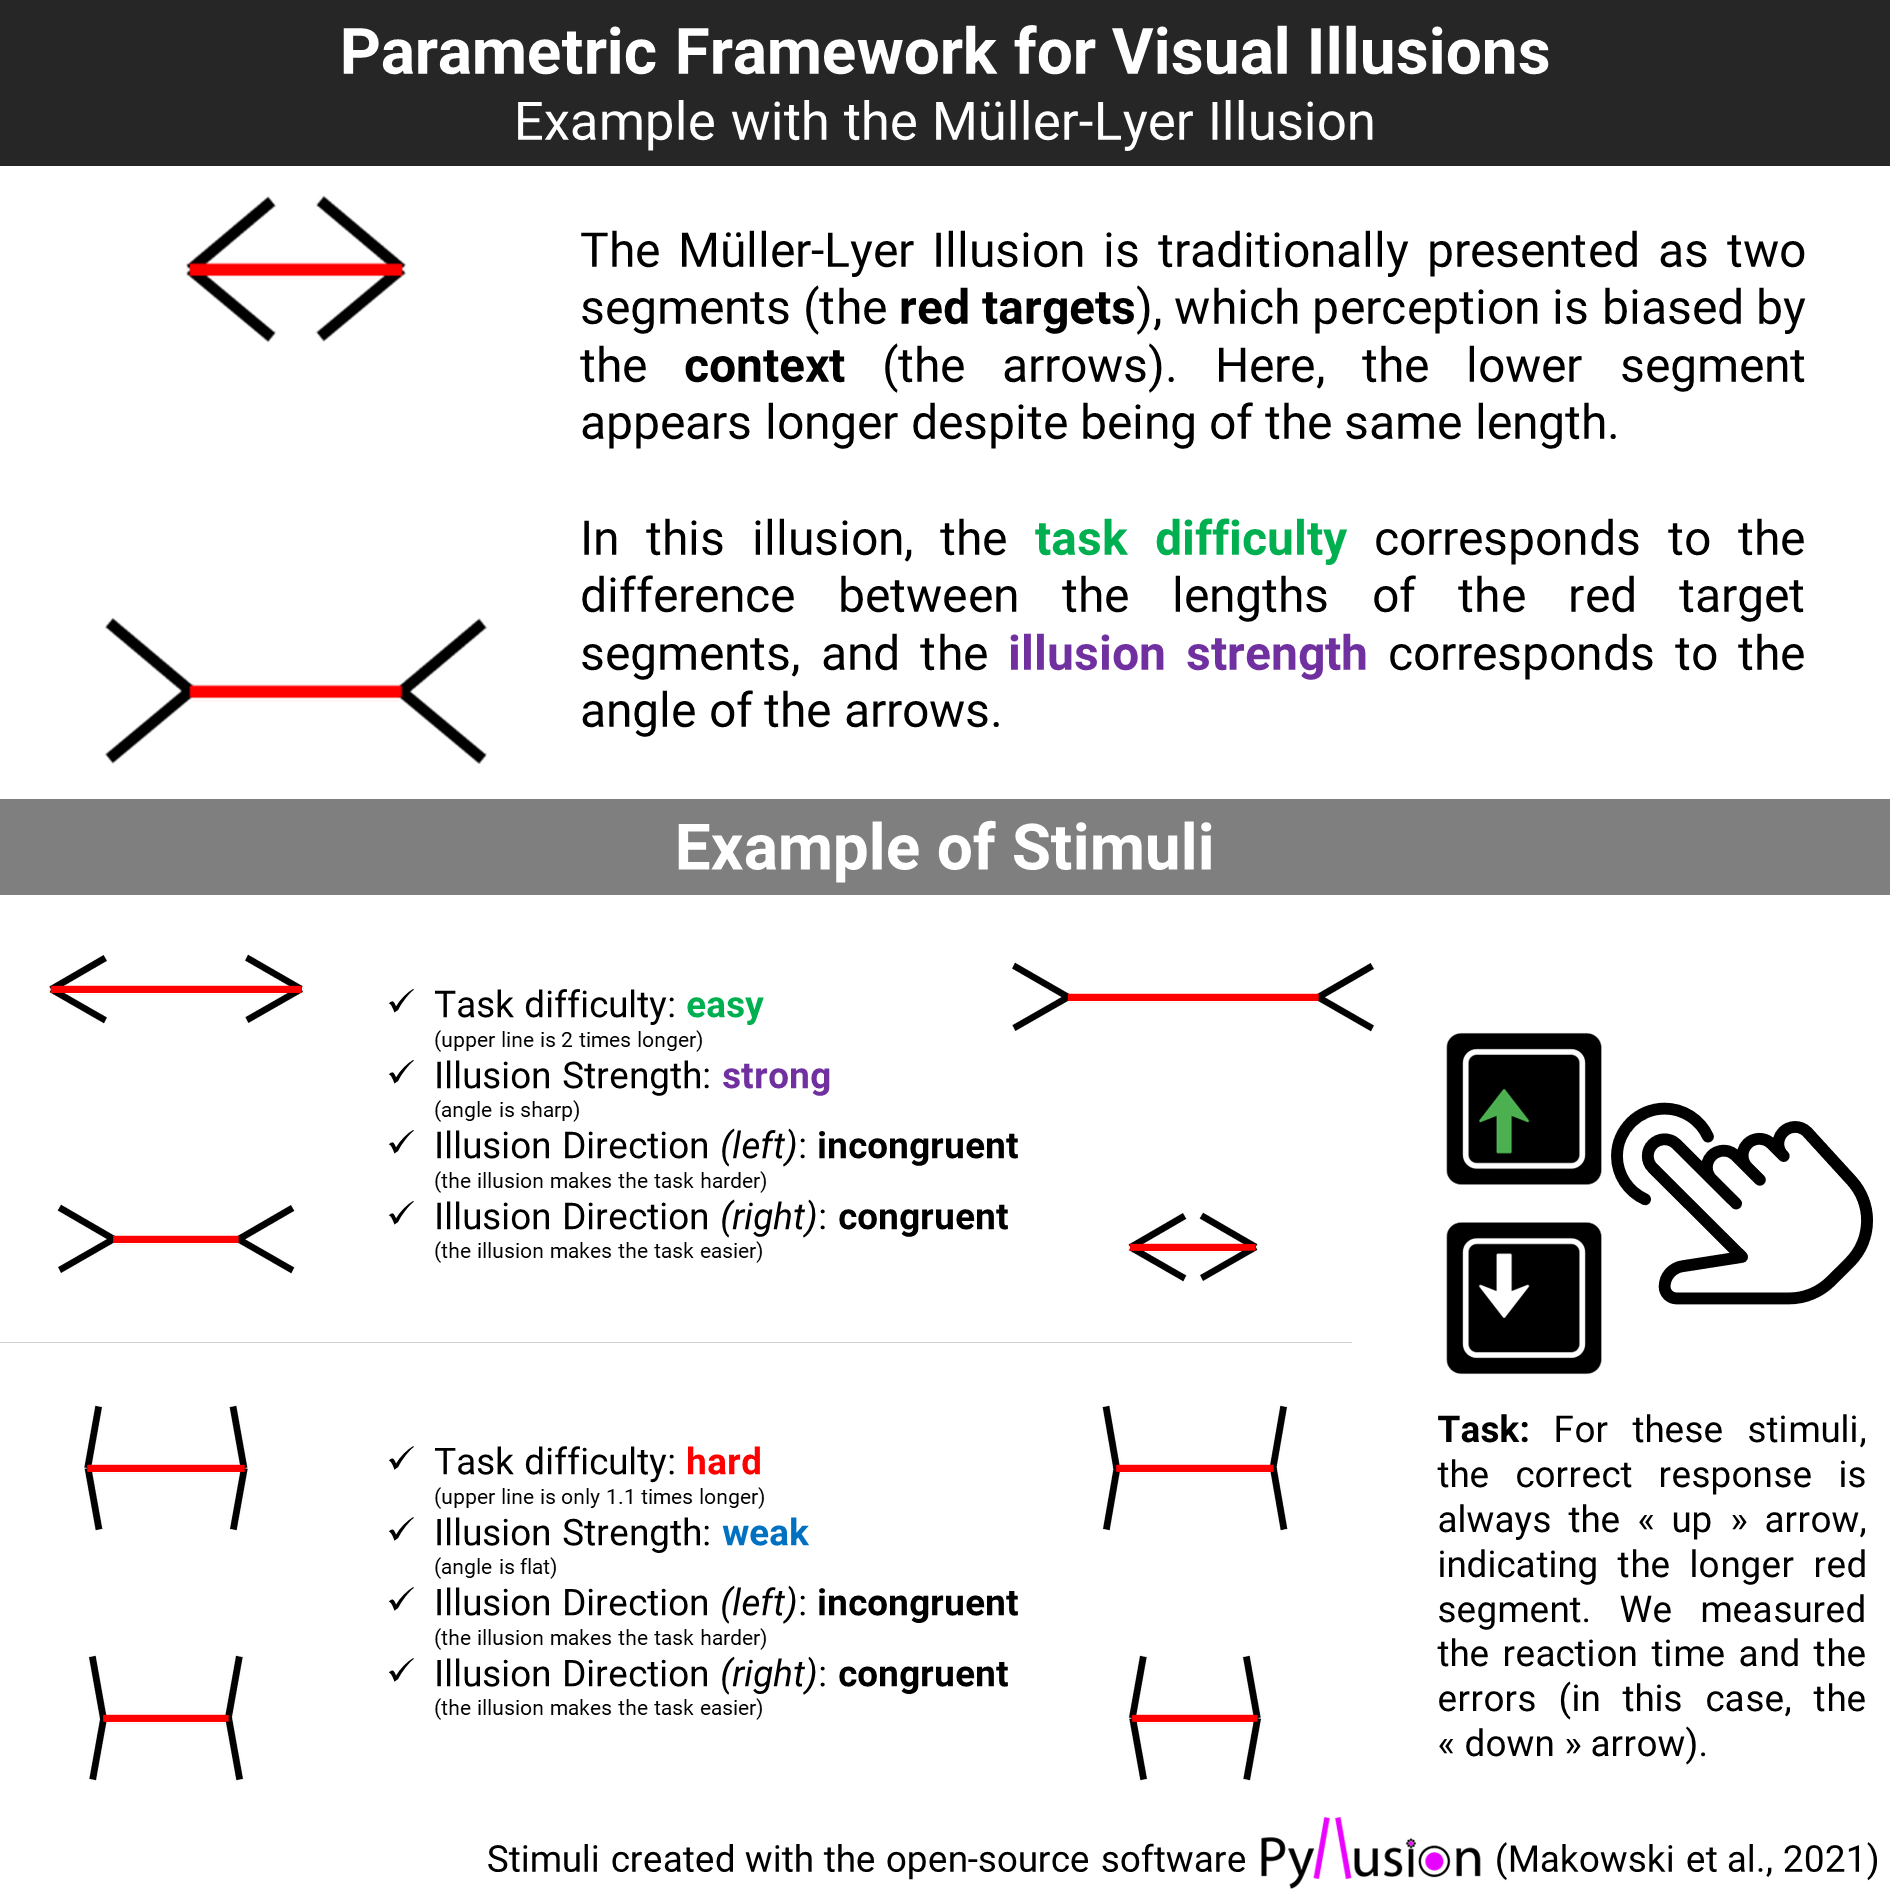
\includegraphics[width=4.2in]{figures/Figure1} \caption{Explanation of the parametric framework for visual illusions (Makowski et al., 2021) applied to the Müller-Lyer illusion (above). Examples of stimuli showcasing the manipulation of the two main parameters, the task difficulty and the illusion strength (below).}\label{fig:unnamed-chunk-2}
\end{figure}

Indeed, many visual illusions can be seen as made of \emph{targets} (e.g., same-length lines), which perception is biased by the \emph{context} (e.g., in the Müller-Lyer illusion, the segments appear of different lengths when they end with inwards or outwards pointing arrows). While most of the paradigms used in the literature prompt the subjective extent the context biases the perception (``how much does the circle appear bigger'', e.g., \textbf{REFS}), \emph{Pyllusions} allows to create illusions in which the targets are actually more or less different (i.e., one segment is longer than the other), and in which the illusion is of varying strength (the arrows are more or less pointy).

This opens the door of an experimental task in which participants have to make perceptual judgments about the targets (e.g., which segment in the longest) under different conditions of objective difficulty and illusion strength. Moreover, the illusion effect can be either ``incongruent'' (making the task even harder by biasing the perception in the opposite way) or ``congruent'' (making the task easier). Although visual illusions are inherently tied to subjective perception, this framework allows a reversal of the traditional paradigm that could quantify the ``objective'' effect of illusions by measuring its behavioral effect (error rate and reaction times) on the performance in a perceptual task.

In the present set of preregistered studies, we will first test this novel paradigm by investigate if the effect of illusion and task difficulty can be manipulated continuously and separated statistically. Then, we will use the paradigm to assess whether 10 different historical illusions (Delboeuf, Ebbinghaus, Rod and Frame, Vertical-Horizontal, Zöllner, White, Müller-Lyer, Ponzo, Poggendorff, Contrast) share a common latent factor (a long-standing debate). Finally, we will investigate how the the inter-individual sensitivity to illusions relates to other characteristics, such as demographic variables and personality.

In line with our full open-access standards, all the material (stimuli generation code, experiment code, raw data, analysis script with complementary figures and analyses, preregistration, etc.) is available at \textbf{\url{https://github.com/RealityBending/IllusionGameValidation}}.

\hypertarget{study-1}{%
\section{Study 1}\label{study-1}}

\hypertarget{aim}{%
\subsection{Aim}\label{aim}}

Study 1 can be seen as a pilot study which goal was to gather some preliminary data to 1) assess whether the stimuli generated by \emph{Pyllusion} behave as expected for each of the 10 illusion types (i.e., increase of task difficulty and illusion strength leading to increased error rate) and 2) develop an intuition of the magnitude of effects, to then refine the stimuli parameters to a sensible range (i.e., not overly easy and not impossible hard).

\hypertarget{procedure}{%
\subsection{Procedure}\label{procedure}}

We generated 56 stimuli for each of the 10 illusion types. These stimuli resulted from the combination of 8 linearly-spread levels levels of task difficulty (e.g., {[}1, 2, 3, 4, 5, 6, 7{]}, where 1 corresponds to the higher difficulty - i.e., the smallest objective difference between targets) and 7 levels of illusion strength (3 values of strength on the congruent side, 3 on the incongruent side, and 0; e.g., {[}-3, -2, -1, 0, 1, 2, 3{]}, where the negative values correspond to congruent illusion strengths).

The 10 illusion blocks were randomly presented, and the order of the 56 stimuli within the block was also randomized. After the first series of 10 blocks, another series was done (with new randomized blocks and trials order). In total, each participant saw 56 different trials per 10 illusion type, repeated 2 times (total = 1120 trials), to which they had to respond ``as fast as possible without making errors'' (i.e., an explicit double constraint to mitigate the inter-individual variability in the speed-accuracy trade off). See instructions for each illusion type in the experiment code.

\hypertarget{participants}{%
\subsection{Participants}\label{participants}}

Fifty-two participants were recruited via \emph{Prolific} (\textbf{REF} about prolific and their data quality) with no restrictions on age or country (the only requisite was a ``fluent'' level of English to match the language of instructions), with a reward of about \textsterling 7.5.

We removed 6 participants upon inspection of the average error rage (when close to 50\%, suggesting random answers), and when the reaction time distribution was implausibly fast. For the remaining participants, we discarded blocks where the error rate was higher than 50\% (possibly indicating that instructions got mixed up; e.g., participants were selecting the shorter line instead of the longer one). Finally, we removed 692 (1.37\%) trials based on an implausibly short or wrong response time (150 ms \textless{} RT \textless{} 3000 ms).

The final sample included 46 participants (Mean age = 26.7, SD = 7.7, range: {[}19, 60{]}; Sex: 39.1\% females, 56.5\% males).

\hypertarget{data-analysis}{%
\subsection{Data Analysis}\label{data-analysis}}

The analysis of study 1 focused on the probability of errors as the main outcome variable. For each illusion, we started by visualizing the average effect of task difficulty and illusion strength to gain some intuition on the underlying generative model. Next, we tested the performance of various models differing in their specifications, such as: with or without a transformation of the task difficulty (log, square root or cubic root), with or without a 2nd order polynomial term for the illusion strength, and with or without the illusion side (up \emph{vs.} down or left \emph{vs.} right) as an additional predictor. We then fitted the best performing model under a Bayesian model, and compared its visualization with that of a General Additive Model (GAM), which has an increased ability of mapping underlying potentially non-linear relationships (at the expense of model simplicity).

The analysis was carried out using \emph{R 4.2} (\textbf{ref}), \emph{brms} (\emph{REF}), the \emph{tidyverse} (\emph{JOSS REF}) and the \emph{easystats} collection of packages (\emph{REFS}).

\hypertarget{results}{%
\subsubsection{Results}\label{results}}

The statistical models suggested that the effect of task difficulty had a cube relationship with error rate for Delboeuf and Ebbinghaus illusions (both based on circle size), square for Rod and Frame, Vertical-Horizontal, cube for Zöllner and Poggendorff, exponential for White, cube for Müller-Lyer and Ponzo (both based on lie lengths), and linear for Contrast. See details and figures in the analysis script.

\hypertarget{discussion}{%
\subsection{Discussion}\label{discussion}}

This study allowed to elaborate a more precise prior idea regarding the magnitude of the effects at stake and the type of interaction between them. It allowed us to better understand and test-out the stimuli generated by \emph{Pyllusion}. It allowed us to uncover a few bugs and issues (for instance, the specification direction of the illusion strength was reversed in the software), which were fixed in a new release.

Crucially, this study allowed us to refine the range of task difficulty and illusion strength values in order to maximize the information gain. One notable result was the illusion effect for the Zöller illusion, which suggested a non-linear pattern. By generating a wider range of illusion strength values, the next study will attempt at clarifying this point.

\hypertarget{study-2}{%
\section{Study 2}\label{study-2}}

\hypertarget{aim-1}{%
\subsection{Aim}\label{aim-1}}

\hypertarget{procedure-1}{%
\subsection{Procedure}\label{procedure-1}}

Perceptual decisions often exhibit a non-linear relationship with the objective physical values (e.g., a logarithmic relationship. In order to spread the difficulty levels based on the behavioral performance (to maximize the diversity of the stimuli in regards to perceptual processes), we generated, for study 2, stimuli with the difficulty levels spaced non-linearly, depending on the best underlying model (i.e., with an exponential, square or cubic spacing if the best model was \emph{log}, \emph{square root} or \emph{cube root}). For instance, a linear space of {[}0.1, 0.3, 0.5, 0.7{]} can be transformed to an exponential space of {[}0.1, 0.27, 0.47, 0.7{]}.

\hypertarget{participants-1}{%
\subsection{Participants}\label{participants-1}}

\hypertarget{general-discussion}{%
\section{General Discussion}\label{general-discussion}}

\hypertarget{future-directions}{%
\section{Future Directions}\label{future-directions}}

We strongly invite researchers to explore and re-analyze our dataset with other approaches and methods to push the understanding further.

\newpage

\hypertarget{references}{%
\section{References}\label{references}}

\hypertarget{refs}{}
\begin{CSLReferences}{0}{0}
\end{CSLReferences}


\clearpage
\renewcommand{\listfigurename}{Figure captions}


\end{document}
